\documentclass[uplatex,dvipdfmx,a4j,12pt]{jsarticle}

\usepackage[utf8]{inputenc}
\usepackage{graphicx}
\usepackage{amsmath}
\usepackage{comment}
\usepackage{color}
\usepackage{url}
\usepackage{siunitx}
\usepackage[version=4]{mhchem}
\usepackage{paralist}
\usepackage{longtable}
\usepackage{multirow}
\usepackage[dvipdfmx]{hyperref}
\usepackage{pxjahyper}
\usepackage{here}
\usepackage{subcaption}

\usepackage{enumitem}
\setlist[description]{parsep=5pt}
\setlist[enumerate]{parsep=5pt}

\title{壁面粗さと壁面$y^+$値について}
\author{14期代空力班長 佐藤空馬}
\date{初版: 2025年5月5日 \\ 最終更新: 2025年9月30日}


\begin{document}
\maketitle

\section{はじめに}

CFDでは,乱流という複雑な流れを計算するために,種々の乱流粘性モデルが提案されている.
大別すれば RANS(Reynolds Averaged Navier-Stokes)モデルとLES(Large Eddy Simulation)モデルに分けられる
\footnote{方程式を直接解くDNS (Direct Numerical Simulation)もあるが,計算コストから一般に現実的でないのでここでは端折る.}.
RANSモデルは渦を平均化することで,比較的荒いメッシュでも計算できるのが特徴である.
LESモデルは,計算格子のサイズよりも大きな渦を直接計算し,それより小さな渦はモデル化することで,より詳細な流れを計算できるモデルであるが,RANSモデルよりも計算コストは増大する.

RANSモデルの中でも幾つか種類があり,代表的なのは,\textbf{$k$-$\varepsilon$モデル} や\textbf{$k$-$\omega$モデル} である.
詳細は省略するが,$k$-$\varepsilon$モデルは計算コストが低いものの壁近傍の流れを捉えるのが苦手であり,$k$-$\omega$モデルは逆に計算コストが高いものの壁近傍の流れを捉えるのが得意であるという特徴がある.
そこで,これらを組み合わせ,壁近傍では$k$-$\omega$モデルを用い,壁から離れた流れでは$k$-$\varepsilon$モデルを用いるという手法が提案されている.
これを\textbf{SST (Shear Stress Transport)モデル}と呼ぶ.
F.T.E.では,このSSTモデルを用いている.

このSSTモデルにおいて,壁近傍の流れを捉えるために,壁面からの距離を無次元化した\textbf{$y^+$}が重要な役割を果たす.
壁面距離の無次元量$y^+$によって,壁近傍における流速の無次元量$u^+$を決定することができる.

以上が乱流粘性モデルと$y^+$の大略である.
詳細は11期の山本さんが書いた「乱流モデルと$y^+$について.pdf」という資料を参照してほしい.

さて,$y^+$は1以下が推奨されるとされている.
実際,\href{https://ansyshelp.ansys.com/public//Views/Secured/corp/v251/en/flu_th/flu_th_sec_turb_sst_add_eq.html}{Fluent Theory Guide | 4.7.2. Transport Equations for the Transition SST Model}の,
4.7.2.2.節において,層流・乱流の遷移を捉えるためには1程度が望ましく,5を超えると遷移点が上流へ移動することがあるとされている
\footnote{なお,参考文献\cite{sst_mesh}によれば,$y^+$値が非常に小さい場合($< 0.001$)にも,遷移点が後流へ移動するために避けるべきであるとされる.}
.
しかし,粗さを考慮したCFDシミュレーションにおいては,$y^+$が1以下になるようにメッシュを細かくすることは非常に困難だった.

そこで,壁面粗さが存在する場合の壁面の取り扱いについて調査したところ,$y^+$が1以下である必要はないことが分かった (正確には,これでは語弊がある).
本稿では,壁面粗さが存在する場合の$y^+$の取り扱いと,適切なインフレーション設定について調査した結果を纏める.

\section{壁面の流速と壁面粗さ}
境界層の内部では,壁面からの距離に応じて流速が変化する.
この流速分布は実験的に次のように与えられることが知られている:
\begin{align}
  \text{粘性底層}(y^+ < 5) & : u^+ = y^+ \\
  \text{乱流層(慣性底層)} (y^+ > 30) & : u^+ = \frac{1}{\kappa} \ln Ey^+ \\
\end{align}
ここで,$\kappa$はフォン・カルマン定数 (0.4187),$E$は経験的な定数(9.793) である.
これを\emph{壁関数}と呼ぶ.
また,特に乱流層における関係を対数則と呼ぶ.

実験的な結果により,粗い壁面近傍の平均流速分布は,semi-logスケールでプロットしたときに,同じ傾き$1/\kappa$を持つが,切片が異なることが分かっている.
つまり,
\begin{equation}
  u^+ = \frac{1}{\kappa} \ln E y^+ - \Delta B
\end{equation}
ここで,$\Delta B$は粗さの影響を表す定数であり,これは壁面の粗さ高さ$K_s$を無次元化して,
\begin{equation}
  K_s^+ = \frac{\rho K_s C_\mu^{1/4}\sqrt{k}}{\mu}.
\end{equation}
とおくと ($C_\mu$は$k$-$\varepsilon$モデルにおける定数0.09,$k$は乱流粘性エネルギー),
\begin{equation}
  \Delta B =
  \begin{cases}
    0 & (K_s^+ < 2.25) \\
    1 / \kappa \ln \left[ \frac{K_s^+ - 2.25}{87,75} + C_s K_s^+ \right] \sin\left\{0.4258(\ln K_s^+ - 0.811)\right\} & (2.25 \leq K_s^+ \leq 90) \\
    1 / \kappa \ln \left( 1 L C_s K_s^+ \right) & (K_s^+ > 90)
  \end{cases}
\end{equation}
となる (ここで,$C_s$は粗さ定数).

細かい定数の定義は端折ったので,気になる人は詳細は参考文献リストをあたってほしい.

\begin{figure}[H]
  \centering
  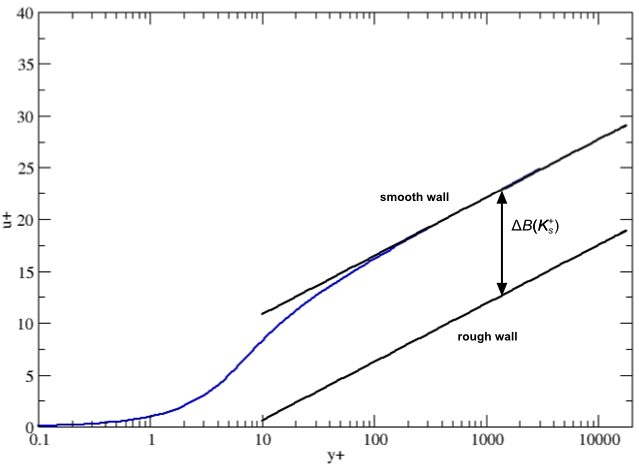
\includegraphics[width=0.8\linewidth]{wall_function/img/g_flu_ug_wall_rough_shift.png}
  \caption{流速の対数プロットとその下方シフト(\cite{wall_model}から図引用).}
  \label{fig:wall_function}
\end{figure}

ここで,壁面の粗さ高さが大きい場合や$y^+$が小さい領域では$u^+$が負になるという特異性が生じることが分かる. 
これでは壁面にめり込んでいることになる(∵ 壁面で0なのでそれより負は壁内)ので,破綻してしまう.

そこで,次の手法が用いられる.

\begin{enumerate}
  \item 壁面粗さを再定義する : $K_s^+ = \min(K_s^+, y^+)$
  \item 壁を仮想的に移動する : $y^+ = y^+ + K_s^+ / 2$
\end{enumerate}

第一の手法については特に言及するまでもなく,またこれからメッシュ要件として$y^+ > K_s^+$が求められる(それ以上はメッシュが過小).

第二の手法については,粘性底層は粗い壁面では表面の凸凹が底層よりも厚くなるために破壊されることに基づいている.
これによって,粗い流れでは粘性底層はなくなり,底層における粘性効果は無視できるようになる.
直径$K_s^+$の球を敷き詰めた等価な砂粒モデルによって考えると,おおよそ高さの半分の領域が流れが阻害されていることが分かる(Blockage Effect).
そこで,実質的な壁面として\textbf{等価砂粒粗さ高さ (equivalent sand-grain roughness height)} を基に計算される$K_s^+ / 2$だけ壁面を移動させることで,表面粗さによる壁面の影響を考慮することができる.
ANSYSでは,$k$-$\omega$モデルや多くの$k$-$\varepsilon$モデルにおいて,このような壁面のシフトによって壁面粗さを計算している.

\section{層流から乱流への遷移と壁面粗さの影響}

また,粗さによって層流から乱流への遷移においても壁面粗さは影響を及ぼす.
ここで重要なのは,等価砂粒粗さ高さではなく,\textbf{幾何的粗さ高さ (geometric roughness height)} である.
このパラメタは粘性モデルダイアログボックスで粗さ相関を有効化することで設定できる.


\section{CFD解析}
% 以上が壁面粗さが壁面$y^+$などに及ぼす影響についての概説である.
この章では,壁面粗さを考慮しない場合/する場合において$y^+$や抗力がどのように変化するか,実際にCFD解析した結果を紹介する.

図\ref{table:setup}に基本的なCFD解析の条件を示す.
機体周辺の境界層厚さを適切に捉え,壁面$y^+$値を十分低くするために,特に機体周りの層状メッシュ (インフレーション) を厚く細かく設定している.

\begin{table}[H]
  \centering
  \begin{tabular}{c|cc}
    \hline\hline
    メッシュ & 基本要素サイズ & 0.25 [m]\\
    \hline
    \multirow{3}{*}{インフレーション} & 層数 & 50\\
    & 成長率 & 1.2\\
    & 厚さ & 0.05 [m]\\
    \hline
    \multirow{2}{*}{サイズコントロール} & ノーズ & 0.0075 [m] \\
    & テール & 0.005 [m] \\
    \hline
    \multirow{6}{*}{シミュレーション} & モデル & choku\_kyoku\_watanabe v1\footnotemark \\
    & 乱流粘性モデル & SST遷移モデル \\
    & 流入速度 & 290 [m/s] \\
    & イテレーション & 300 - 400\\
    & 幾何的粗さ高さ & 60 [\textmu m] \\  
    & 等価砂粒粗さ高さ & 60 [\textmu m]\\
    \hline\hline
  \end{tabular}
  \caption{CFD解析の条件}
  \label{table:setup}
\end{table}
\footnotetext{ignisフィン確定後モデル.}

\subsection{壁面粗さを考慮しない場合/する場合の$y^+$値と抗力係数}
壁面粗さを考慮しない場合の,壁面$y^+$値の分布を示す.
\begin{figure}[H]
  \centering
  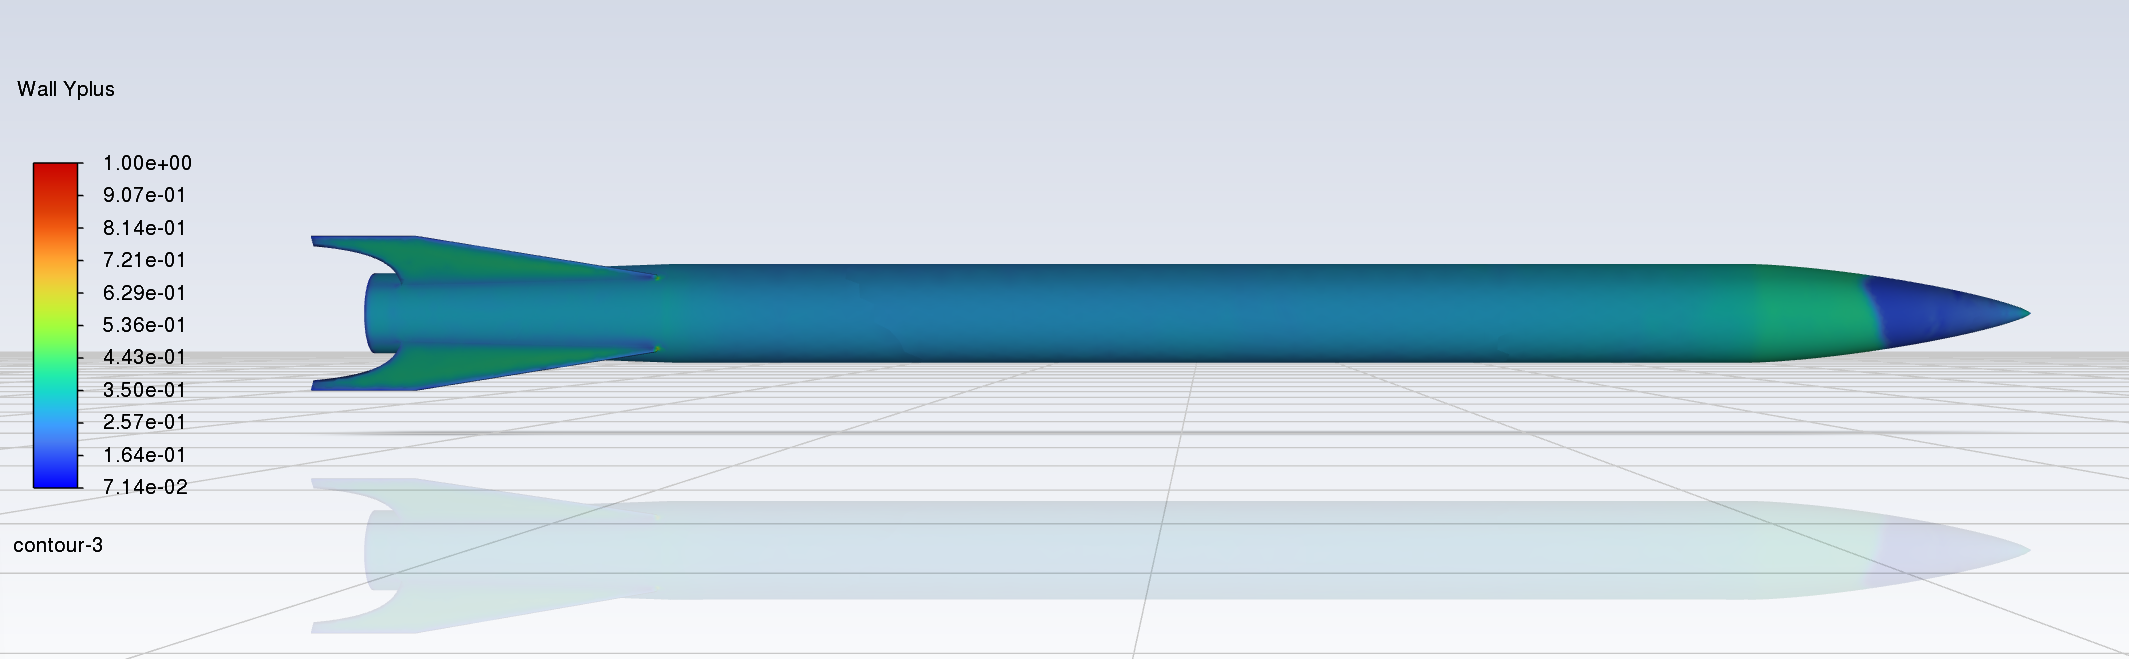
\includegraphics[width=\linewidth]{wall_function/img/4_1_yplus_wo_rough.png}
  \caption{壁面$y^+$値の分布 (壁面粗さを考慮しない場合)}
  \label{fig:yplus_no_rough}
\end{figure}
機体表面で$y^+$値が1以下であることが分かる.

一方で,壁面粗さを考慮した場合の壁面$y^+$値の分布を図\ref{fig:yplus_rough}に示す.
\begin{figure}[H]
  \centering
  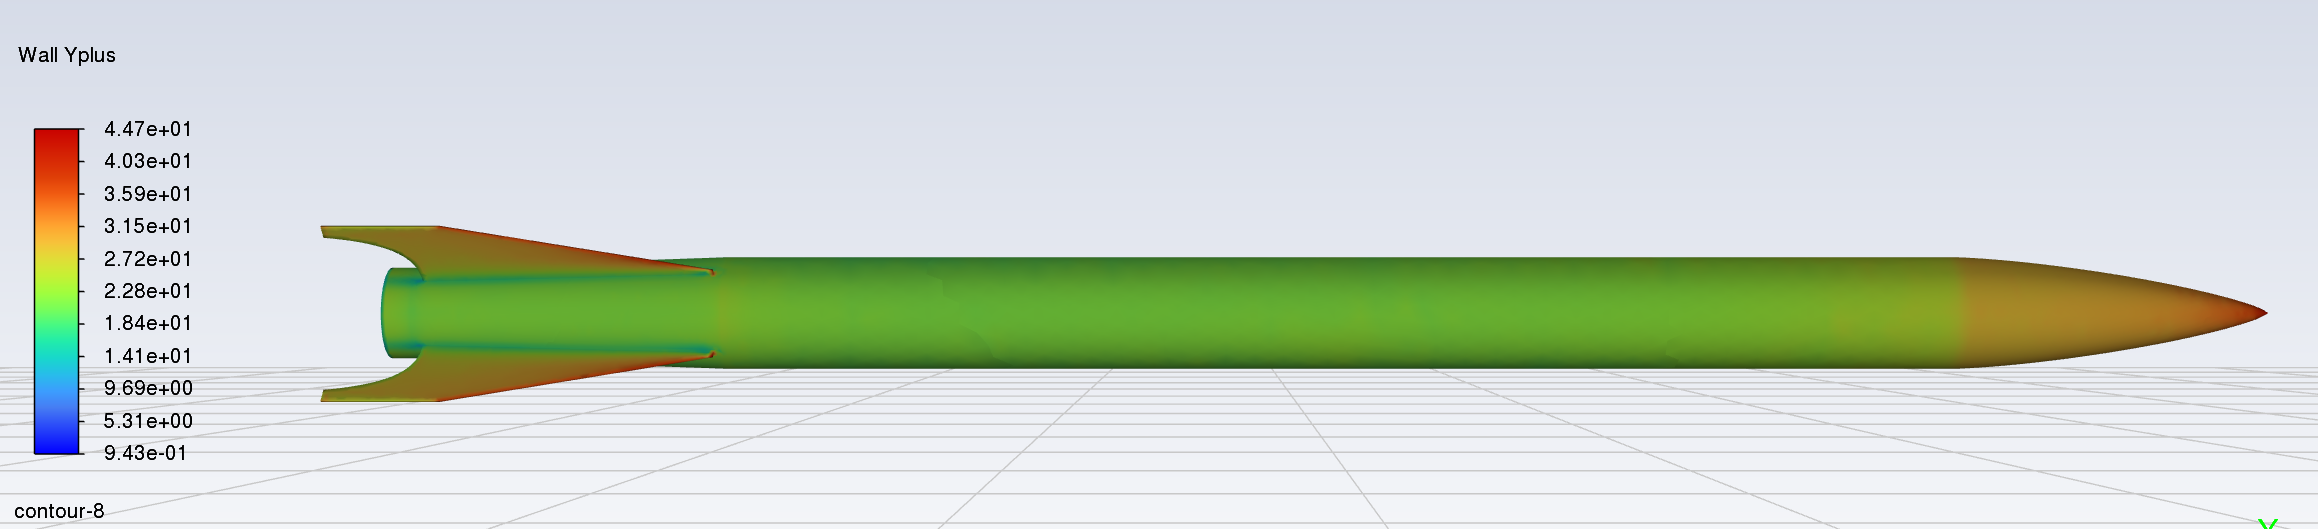
\includegraphics[width=\linewidth]{wall_function/img/4_1_yplus_w_rough.png}
  \caption{壁面$y^+$値の分布 (壁面粗さを考慮する場合)}
  \label{fig:yplus_rough}
\end{figure}
壁面粗さを考慮する場合,壁面$y^+$値は約20程度であり,ノーズやフィンの前縁部では40程度にも達することが分かる.

$K_s^+ = \rho K_s C_\mu^{1/4}\sqrt{k} / \mu$より,この値をAnsys上で計算し
\footnote{
計算は ユーザー定義 $>$ フィールド関数 $>$ ユーザー定義フィールド関数カリキュレータ よりユーザ指定変数を作成することで行える.
$K_s^+$の計算式は,\texttt{density * 0.09 \^\, 0.25 * 6 * 10 \^\, ( - 5) * sqrt (turb-kinetic-energy) / viscosity-lam}
とした (ここで\texttt{viscosity-lam}はPropertiesのMolecular Viscosity).
}
,プロットした結果が図\ref{fig:K_s}である.
これの1/2は凡そ壁面$y^+$値と一致することが分かる.
\begin{figure}[H]
  \centering
  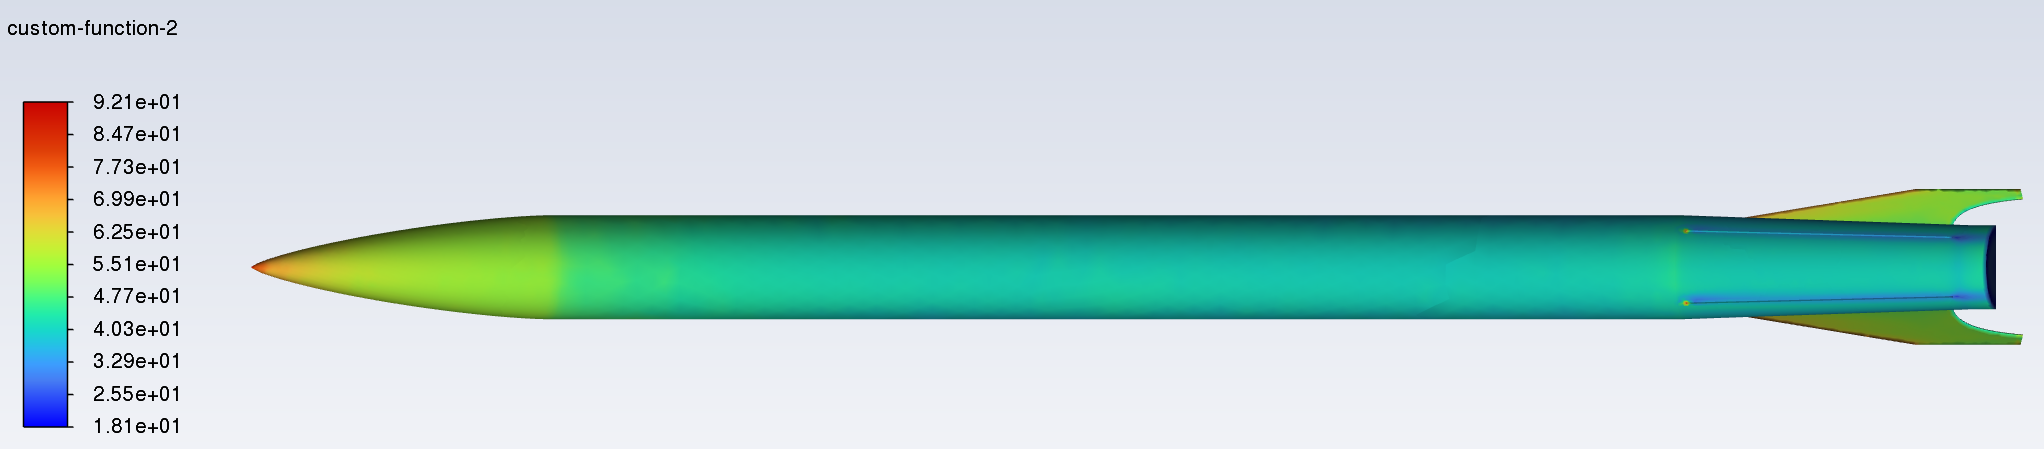
\includegraphics[width=\linewidth]{wall_function/img/4_1_Ksplus.png}
  \caption{粗さ高さ$K_s^+$の分布 (壁面粗さを考慮する場合)}
  \label{fig:K_s} 
\end{figure}

なお,計算の妥当性の補足として,機体表面の速度分布をメッシュと共に図\ref{fig:velocity}に示す.
\begin{figure}[H]
  \centering
  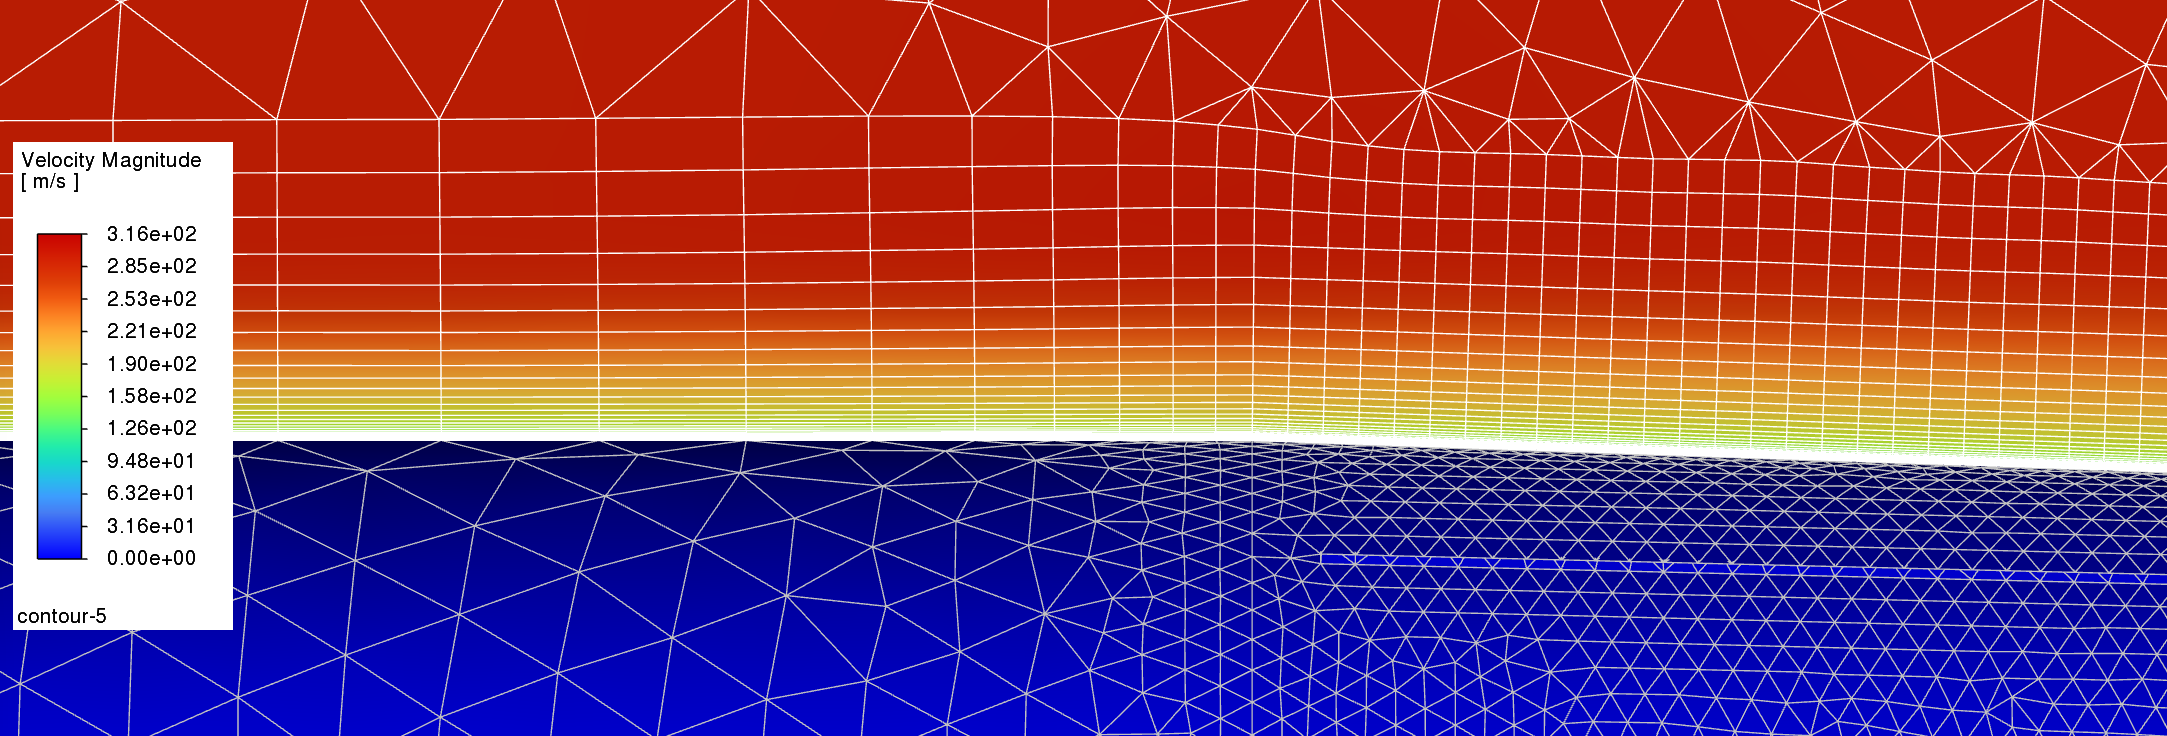
\includegraphics[width=\linewidth]{wall_function/img/4_1_velocity.png}
  \caption{機体表面の速度分布 (フィン前縁部付近,壁面粗さを考慮しない場合)}
  \label{fig:velocity}
\end{figure}
フィン前縁部付近 (テール前端付近) のような後流部では乱流境界層が十分卓越するが,このような場所においても層状メッシュ内部に乱流境界層が収まっていることが分かる.
したがって,機体周囲の低速部を先のインフレーション設定によって十分適切に捉えられていると言える.
図に示したのは表面粗さを考慮しない場合であったが,考慮した場合でもほぼ同様である.

また,以下の図\ref{fig:4_1_cd}に機体にかかる抗力係数を示す.
機体表面粗さを考慮することで,圧力抵抗は減少するが,粘性抵抗は増大し,系全体のとしては抗力が増大することが分かった.
圧力抵抗が減少した要因としては,表面粗さによって遷移点が前方に移動したため,より剥離しにくくなったことが考えられる.
また,これによって増大する乱流域においては速度勾配が大きいことや,仮想的な壁面のシフト,
粗さによってせん断応力が増大することが
\footnote{自明な気がするが,明確な典拠は見つからなかった.}
粘性抵抗が増大した要因と考えられる.
\begin{figure}[H]
  \centering
  \begin{minipage}{0.45\linewidth}
      \centering
      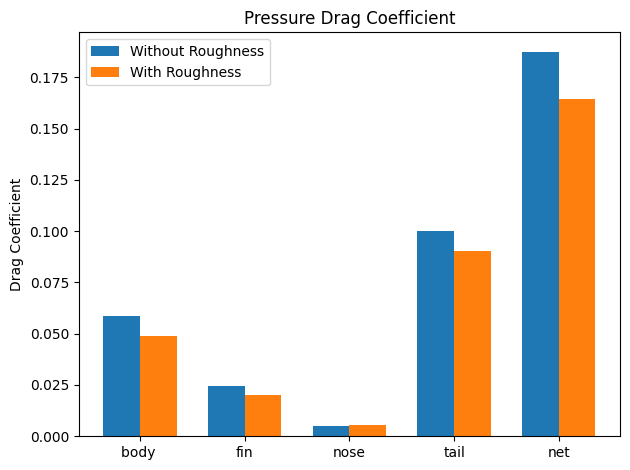
\includegraphics[width=\linewidth]{wall_function/img/4_1_pressure_drag.png}
      \subcaption{圧力抗力係数.}
      \label{fig:4_1_cd_pressure}
  \end{minipage}
  \begin{minipage}{0.45\linewidth}
      \centering
      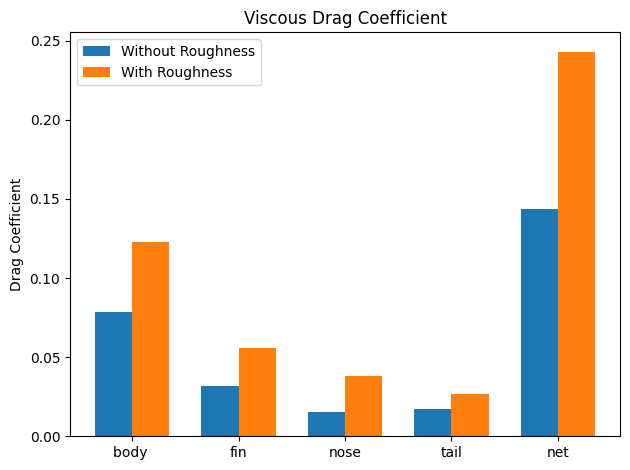
\includegraphics[width=\linewidth]{wall_function/img/4_1_viscous_drag.png}
      \subcaption{粘性抗力係数.}
      \label{fig:4_1_cd_viscous}
  \end{minipage}
  \begin{minipage}{0.45\linewidth}
      \centering
      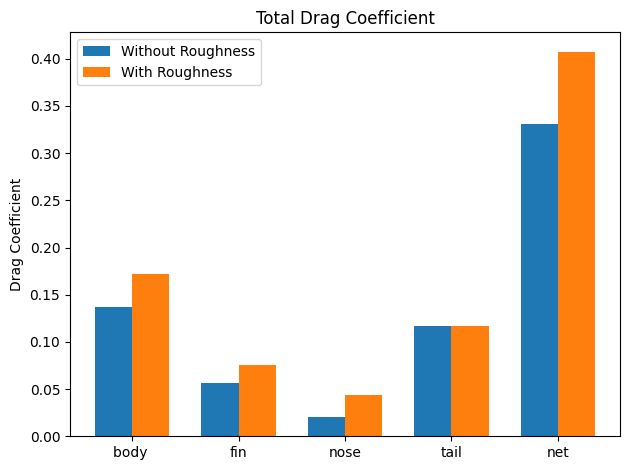
\includegraphics[width=\linewidth]{wall_function/img/4_1_total_drag.png}
      \subcaption{全抗力係数.}
      \label{fig:4_1_cd_total}
  \end{minipage}
  \caption{表面粗さを考慮しない場合/する場合の抗力係数の比較.}
  \label{fig:4_1_cd}
\end{figure}


\subsection{不適切なインフレーションの場合 --- 厚さについて ---}
次に,インフレーションを境界層厚さよりも薄い 0.001 [m] に設定した場合に,壁面$y^+$値分布や抗力係数がどのように変動するかを示す.
ここでは$y^+$値を1以下に設定するために,層数は25に設定した.

まず始めに,壁面粗さを考慮しない場合の壁面$y^+$値分布を図\ref{fig:yplus_no_rough_2}に示す.
\begin{figure}[H]
  \centering
  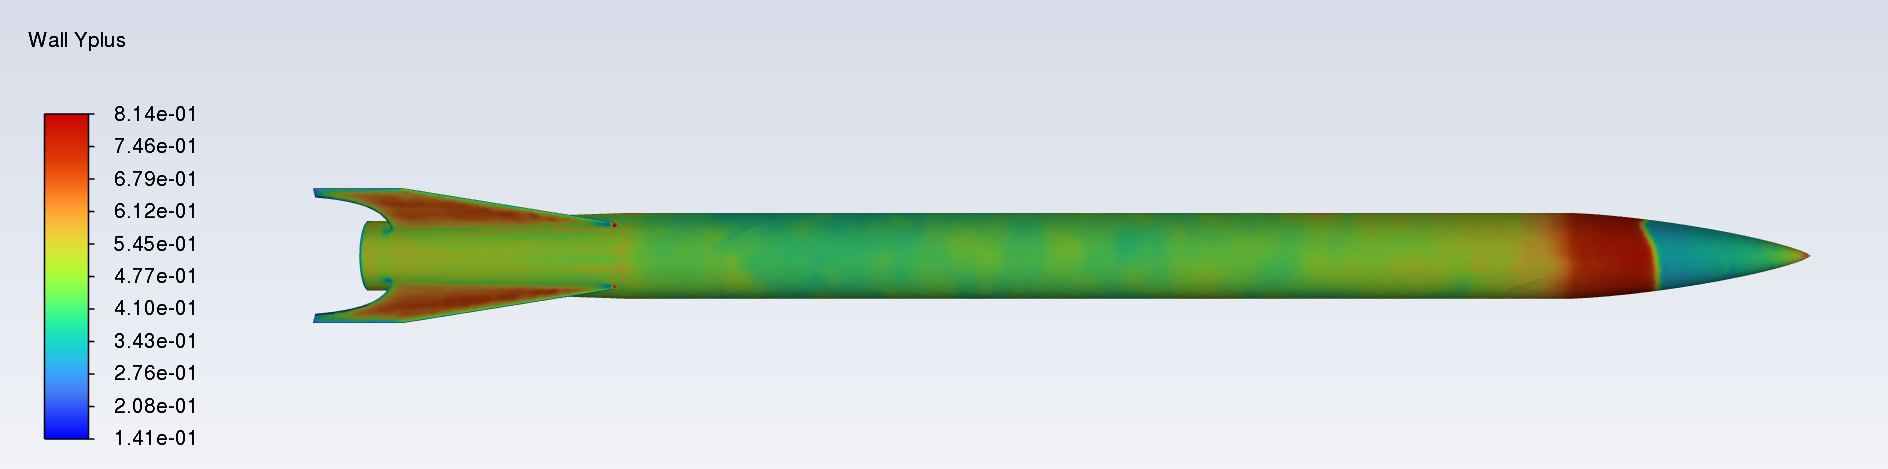
\includegraphics[width=\linewidth]{wall_function/img/4_2_yplus.png}
  \caption{壁面$y^+$値の分布 (壁面粗さを考慮しない場合)}
  \label{fig:yplus_no_rough_2}
\end{figure}

なお,機体表面の流速分布とメッシュの様子を図\ref{fig:velocity_2}に示す.
\begin{figure}[H]
  \centering
  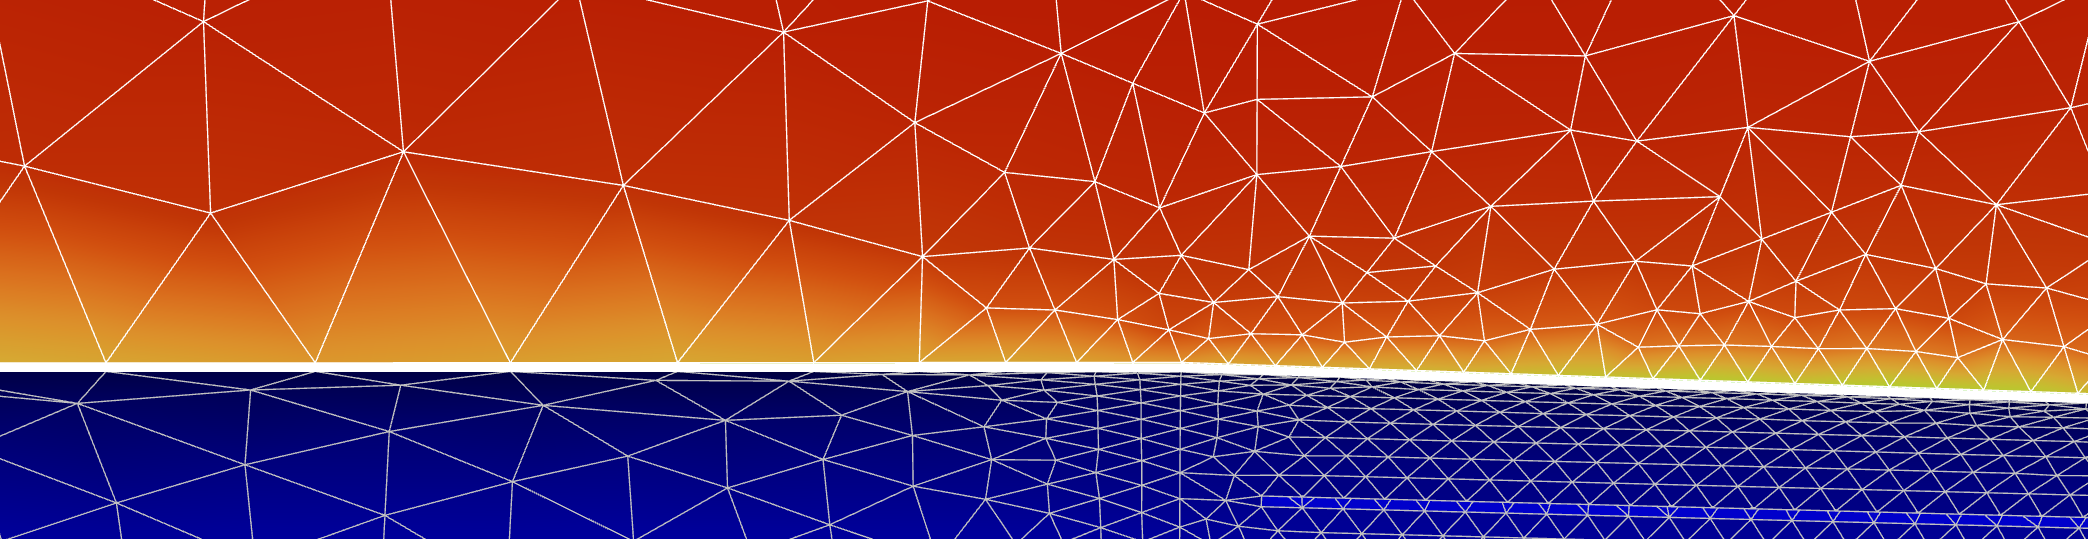
\includegraphics[width=\linewidth]{wall_function/img/4_2_velocity.png}
  \caption{機体表面の速度分布 (フィン前縁部付近,壁面粗さを考慮しない場合)}
  \label{fig:velocity_2}
\end{figure}

抗力係数について,適切にメッシュを設定した場合 (図\ref{fig:4_1_cd}) と比較した結果を図\ref{fig:4_1_cd_wo_rough}, 図\ref{fig:4_2_cd_w_rough}に示す.
表面粗さを考慮する場合/しない場合の両方において圧力抗力係数に大きな変化は見られなかったが,粘性抗力係数は不適切なインフレーション厚さにおいて大きく減少した.
これは,インフレーション厚さが薄いために,特にインフレーション最外部--境界層最外部間において速度勾配が緩やかになったことに起因すると考えられる.

\begin{figure}[H]
  \centering
  \begin{minipage}{0.45\linewidth}
      \centering
      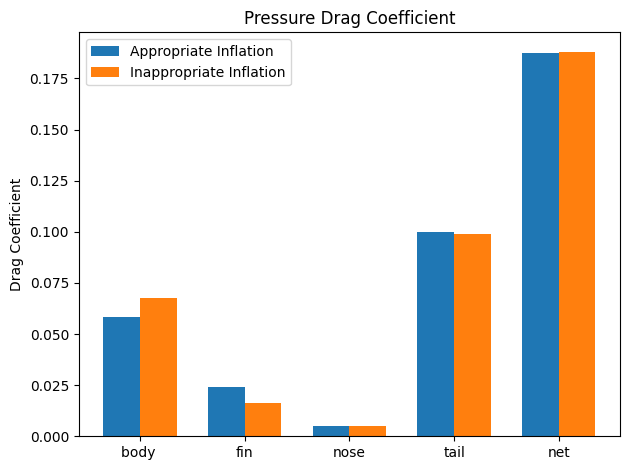
\includegraphics[width=\linewidth]{wall_function/img/4_2_2_pressure_drag.png}
      \subcaption{圧力抗力係数.}
      \label{fig:4_2_2_cd_pressure}
  \end{minipage}
  \begin{minipage}{0.45\linewidth}
      \centering
      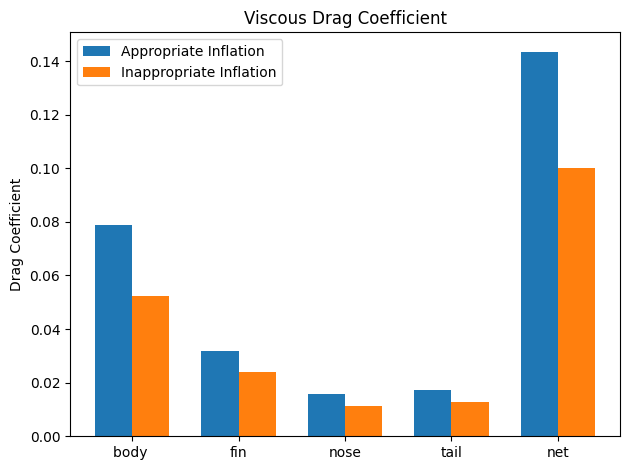
\includegraphics[width=\linewidth]{wall_function/img/4_2_2_viscous_drag.png}
      \subcaption{粘性抗力係数.}
      \label{fig:4_2_2_cd_viscous}
  \end{minipage}
  \begin{minipage}{0.45\linewidth}
      \centering
      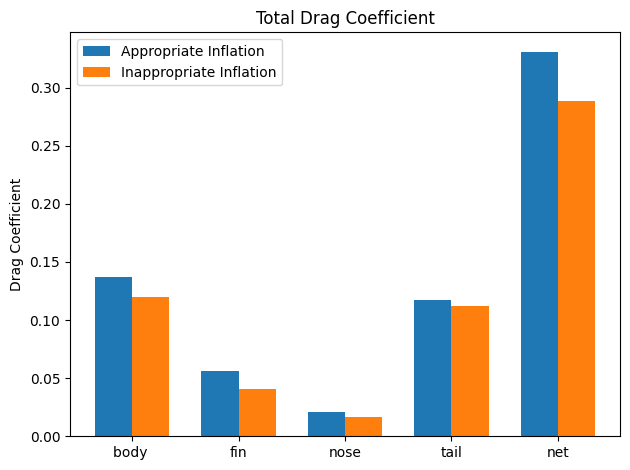
\includegraphics[width=\linewidth]{wall_function/img/4_2_2_total_drag.png}
      \subcaption{全抗力係数.}
      \label{fig:4_2_2_cd_total}
  \end{minipage}
  \caption{インフレーション厚さが適切/不適切な場合の抗力係数の比較(粗さなし).}
  \label{fig:4_2_cd_wo_rough}
\end{figure}

\begin{figure}[H]
  \centering
  \begin{minipage}{0.45\linewidth}
      \centering
      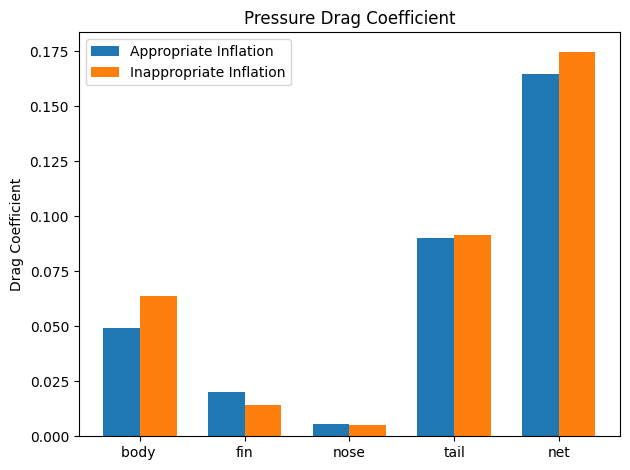
\includegraphics[width=\linewidth]{wall_function/img/4_2_1_pressure_drag.png}
      \subcaption{圧力抗力係数.}
      \label{fig:4_2_1_cd_pressure}
  \end{minipage}
  \begin{minipage}{0.45\linewidth}
      \centering
      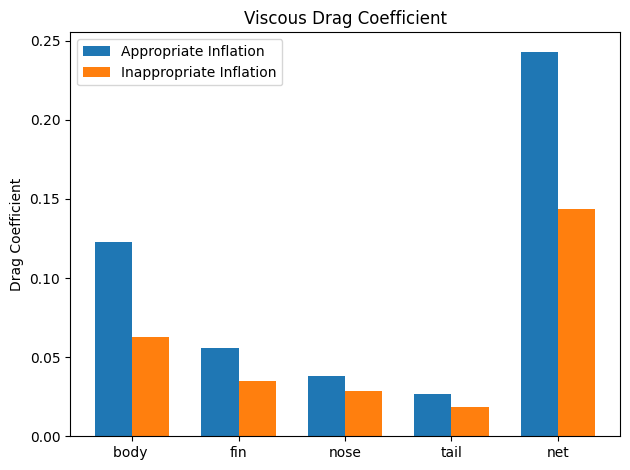
\includegraphics[width=\linewidth]{wall_function/img/4_2_1_viscous_drag.png}
      \subcaption{粘性抗力係数.}
      \label{fig:4_2_1_cd_viscous}
  \end{minipage}
  \begin{minipage}{0.45\linewidth}
      \centering
      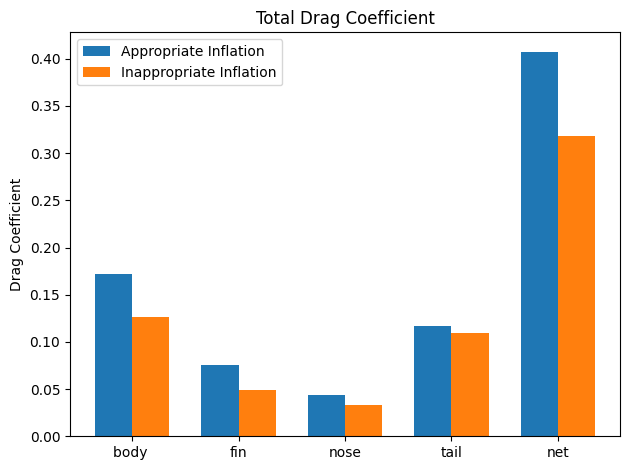
\includegraphics[width=\linewidth]{wall_function/img/4_2_1_total_drag.png}
      \subcaption{全抗力係数.}
      \label{fig:4_2_1_cd_total}
  \end{minipage}
  \caption{インフレーション厚さが適切/不適切な場合の抗力係数の比較(粗さあり).}
  \label{fig:4_2_cd_w_rough}
\end{figure}

\subsection{不適切なインフレーションの場合 --- 層数について ---}
次に,層数を50から25に減らした場合に壁面$y^+$値分布や抗力係数がどのように変動するかを示す.
ここでは,インフレーション厚さは0.05 [m] に設定した.

まず始めに,壁面粗さを考慮しない場合の壁面$y^+$値分布と流速分布を図\ref{fig:yplus_no_rough_3},図\ref{fig:velocity_3}に示す.
適切に機体周囲の低速域を捉えられている一方で,壁面$y^+$値はボディ部で70程度,ノーズ部では100程度に達していることが分かる.
\begin{figure}[H]
  \centering
  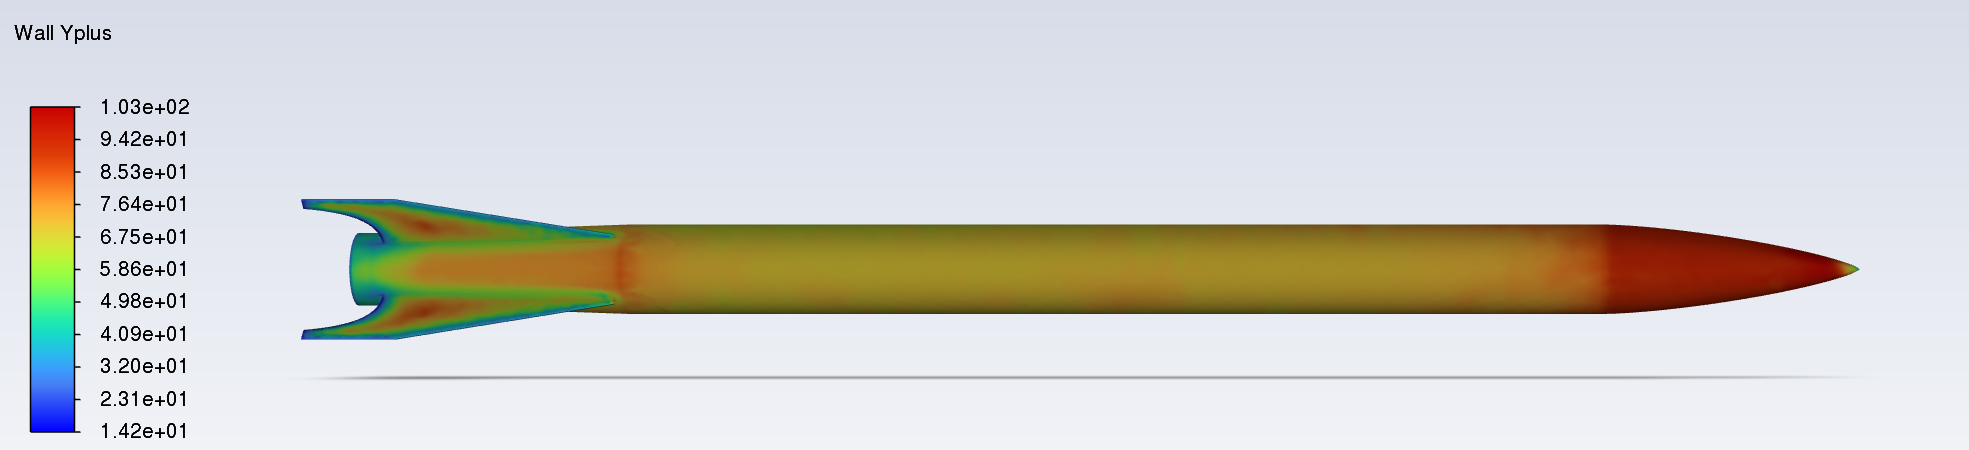
\includegraphics[width=\linewidth]{wall_function/img/4_3_yplus.png}
  \caption{壁面$y^+$値の分布 (壁面粗さを考慮しない場合)}
  \label{fig:yplus_no_rough_3}
\end{figure}

\begin{figure}[H]
  \centering
  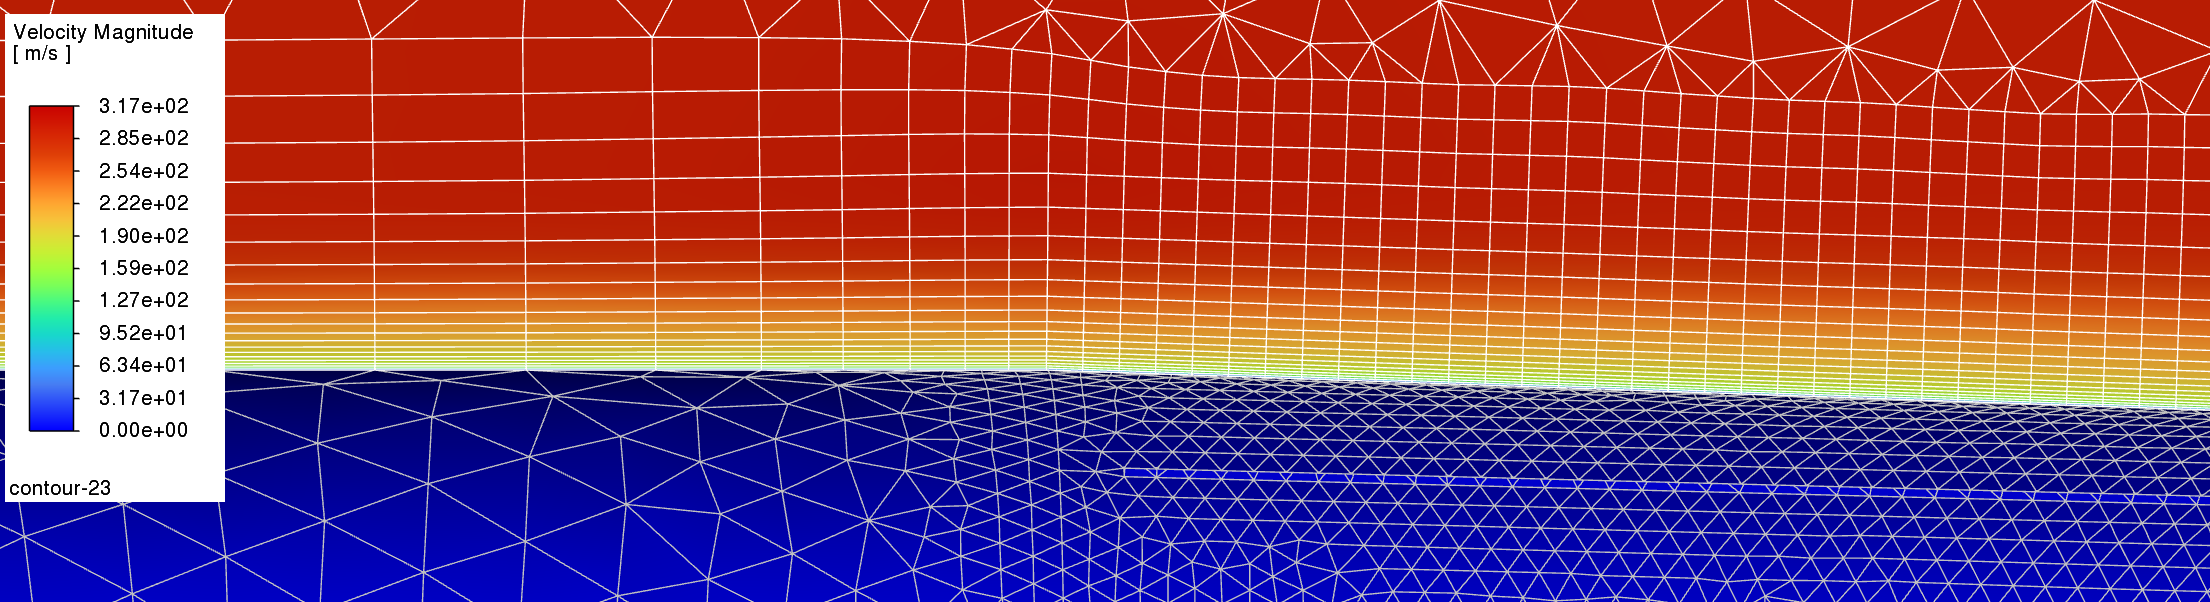
\includegraphics[width=\linewidth]{wall_function/img/4_3_velocity.png}
  \caption{機体表面の速度分布 (フィン前縁部付近,壁面粗さを考慮しない場合)}
  \label{fig:velocity_3}
\end{figure}

抗力係数を適切にメッシュを設定した場合 (図\ref{fig:4_1_cd}) と比較した結果を図\ref{fig:4_3_cd_wo_rough}, 図\ref{fig:4_3_cd_w_rough}に示す.
この場合においては,圧力抵抗のみが低減し,粘性抵抗には変化が見られなかった.
これは,$y^+$値が5よりも大きいため,乱流への遷移点が前方に移動したことで,剥離が起こりにくくなったことが要因と考えられる.
また,粘性抵抗に影響は見られなかったことから,速度勾配については25層のインフレーションでも十分適切に捉えられていることが予想される
\footnote{粘性抵抗に変化が見られないことから,乱流域の増大による粘性抵抗の増大はない可能性が示唆される.
この場合,粘性抵抗が粗さを考慮することで増大した要因として,乱流域の増大を挙げるのは不適切に思える.
すなわち,それ以外の要因 (せん断応力の増大や壁面のシフト) の寄与の方が大きいと考えられる.
}
.

\begin{figure}[H]
  \centering
  \begin{minipage}{0.45\linewidth}
      \centering
      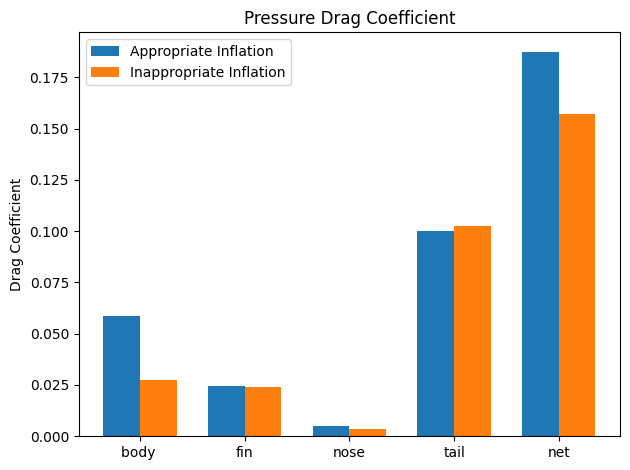
\includegraphics[width=\linewidth]{wall_function/img/4_3_2_pressure_drag.png}
      \subcaption{圧力抗力係数.}
      \label{fig:4_3_2_cd_pressure}
  \end{minipage}
  \begin{minipage}{0.45\linewidth}
      \centering
      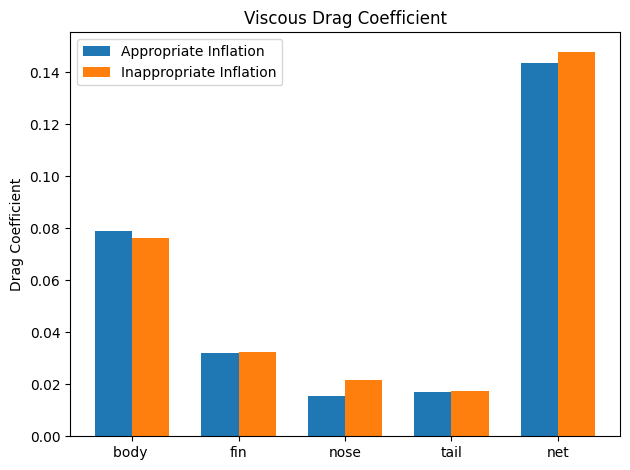
\includegraphics[width=\linewidth]{wall_function/img/4_3_2_viscous_drag.png}
      \subcaption{粘性抗力係数.}
      \label{fig:4_3_2_cd_viscous}
  \end{minipage}
  \begin{minipage}{0.45\linewidth}
      \centering
      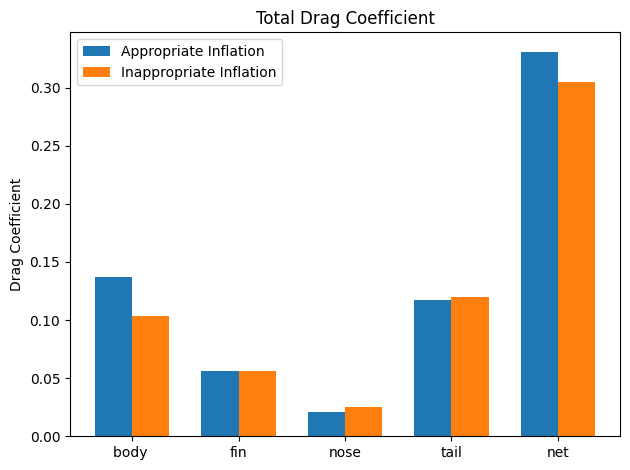
\includegraphics[width=\linewidth]{wall_function/img/4_3_2_total_drag.png}
      \subcaption{全抗力係数.}
      \label{fig:4_3_2_cd_total}
  \end{minipage}
  \caption{インフレーションの層数が適切/不適切な場合の抗力係数の比較(粗さなし).}
  \label{fig:4_3_cd_wo_rough}
\end{figure}

\begin{figure}[H]
  \centering
  \begin{minipage}{0.45\linewidth}
      \centering
      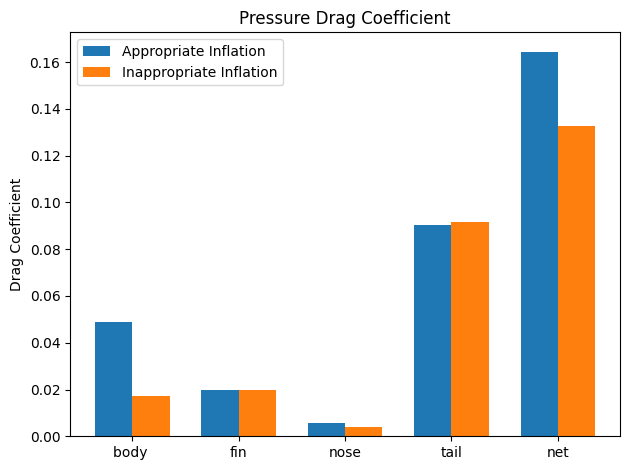
\includegraphics[width=\linewidth]{wall_function/img/4_3_1_pressure_drag.png}
      \subcaption{圧力抗力係数.}
      \label{fig:4_3_1_cd_pressure}
  \end{minipage}
  \begin{minipage}{0.45\linewidth}
      \centering
      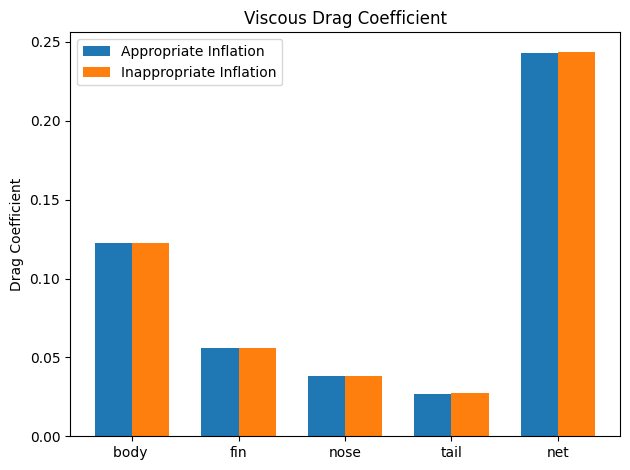
\includegraphics[width=\linewidth]{wall_function/img/4_3_1_viscous_drag.png}
      \subcaption{粘性抗力係数.}
      \label{fig:4_3_1_cd_viscous}
  \end{minipage}
  \begin{minipage}{0.45\linewidth}
      \centering
      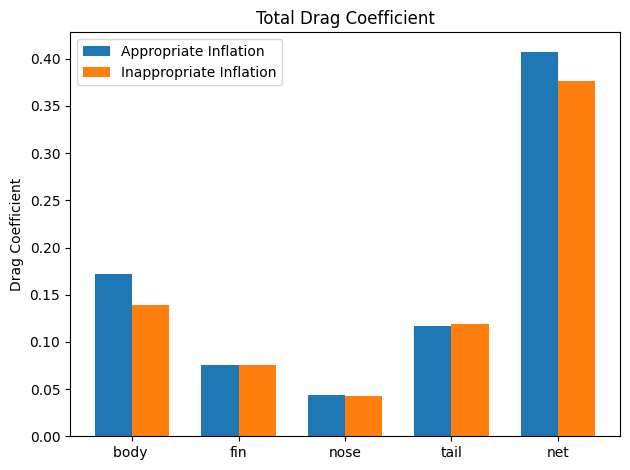
\includegraphics[width=\linewidth]{wall_function/img/4_3_1_total_drag.png}
      \subcaption{全抗力係数.}
      \label{fig:4_3_1_cd_total}
  \end{minipage}
  \caption{インフレーションの層数が適切/不適切な場合の抗力係数の比較(粗さあり).}
  \label{fig:4_3_cd_w_rough}
\end{figure}

\section{結論}
本稿では,壁面粗さが壁面$y^+$や遷移などに及ぼす影響についての概説を行った.
また,CFD解析を行うことで,壁面$y^+$値や抗力係数がどのように変化するかを調査した.
その結果,適切にインフレーション設定を行った場合でも,壁面粗さを考慮することで壁面のシフトによって壁面$y^+$値が増大することが分かった.
さらに,その変動量をAnsys上で見積もり,壁面$y^+$の変動量と一致することを確かめた.
また,不適切なインフレーション厚さでは粘性抵抗が,不適切なインフレーション層数では圧力抵抗がそれぞれ減少することが分かった.
このことから,表面粗さを考慮した解析を適切に行うためには,次の順序でCFD解析を行うことが望ましいと考えられる:
\begin{enumerate}
  \item 表面粗さを考慮せずにCFD解析を行う.\\
  このとき,壁面$y^+$値が1程度 (5以下) であるか,境界層がインフレーション厚さよりも十分薄いか確認する.
  \item 表面粗さを考慮してCFD解析を行う.\\
  同様にして,インフレーション内部に境界層が収まっているか確認する.また,気になる場合は$K_s^+$の値を確認する.
\end{enumerate}




\begin{thebibliography}{9}
  \bibitem{sst_mesh}
    \href{https://ansyshelp.ansys.com/public///Views/Secured/corp/v251/en/flu_th/flu_th_sec_turb_sst_grid.html}{Fluent Theory Guide | 4.7.3. Mesh Requirements}. Ansys (2025), (閲覧日:2025年5月5日).

  \bibitem{wall_model}
    \href{https://ansyshelp.ansys.com/public//Views/Secured/corp/v251/en/flu_th/ch04s18s02.html}{Fluent Theory Guide | 4.18.2. Wall Treatment for ε-based Models}. Ansys (2025), (閲覧日:2025年5月5日).
  
  \bibitem{turbulance}
    \href{https://ansyshelp.ansys.com/public//Views/Secured/corp/v251/en/flu_th/x1-5720008.164.html}{Fluent Theory Guide | 4.18.5. Wall Roughness Effects in Turbulent Wall-Bounded Flows}. Ansys (2025), (閲覧日:2025年5月5日).
  
\end{thebibliography}

\section*{改訂履歴}

\begin{table}[H]
  \centering
  \begin{tabular}{c|c|l}
    \hline
    改訂 & 日付 & 内容 \\
    \hline\hline
    1.0 & 2025/05/05 & 初版作成 \\
    1.1 & 2025/09/30 & 誤字修正 \\
    \hline
  \end{tabular}
\end{table}

\end{document}